\documentclass{article}

\usepackage{xcolor}
\usepackage{colortbl}
\usepackage{graphicx}
\usepackage[margin=2cm]{geometry}
\usepackage{verbatim}
\usepackage[export]{adjustbox}

\begin{document}

\newcommand{\code}[1]{\texttt{#1}}
\newcommand{\pct}[1]{$#1\,\%$}
\newcommand{\modefont}[1]{\texttt{#1}}
\newcommand{\mnocheck}{\modefont{nocheck}}
\newcommand{\mnonstrict}{\modefont{nonstrict}}
\newcommand{\mstrict}{\modefont{strict}}
\newcommand{\gcell}[1]{\cellcolor{green!20}#1}
\newcommand{\ycell}[1]{\cellcolor{yellow!18}#1}
\newcommand{\ocell}[1]{\cellcolor{orange!29}#1}
\newcommand{\rcell}[1]{\cellcolor{red!30}$\!\!$#1$\!\!$}
\newcommand{\zerowidth}[1]{\makebox[0pt][l]{#1}}

%% ---
\subsection*{Figure 3: Records per Hour}

Plot from \texttt{code/row-distribution.rkt}, which uses the dataset
\texttt{out/row-distribution.rktd}, which comes from running
\texttt{prepare.rkt --mode main}.

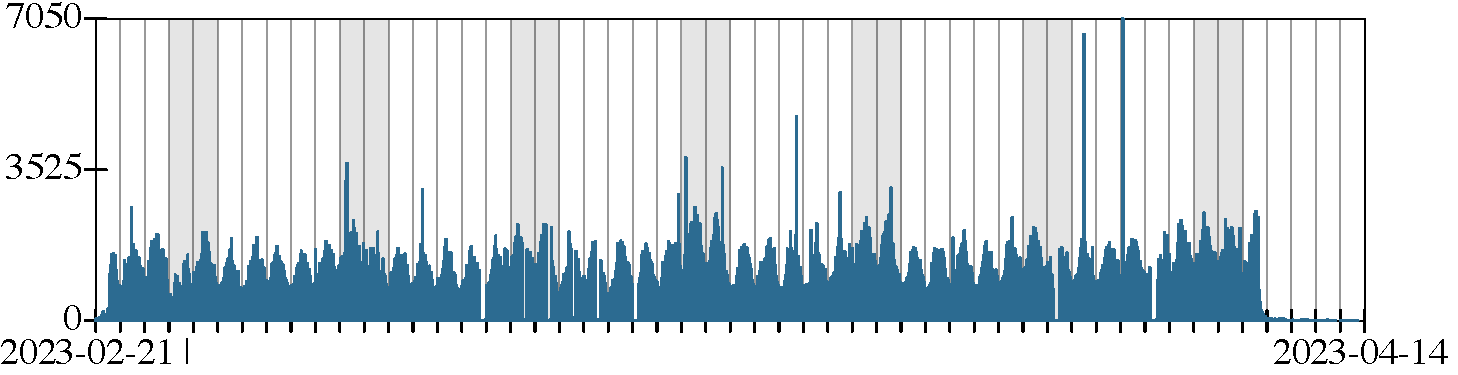
\includegraphics[width=\columnwidth]{out/row-distribution.pdf}

Lines 1-2 of \texttt{out/overview.txt} (output of \texttt{prepare.rkt --mode main})
give the reason for sending:

\begin{verbatim}
 1504736 total logs = 1341348 nocheck + 156883 nonstrict + 6505 strict
  508572 due to module switch
\end{verbatim}


%% ---
\subsection*{Table 2: Size of Analyzed Code}

From \texttt{out/summary-of-size-distributions.rktd},\\
which is the output of \texttt{code/sdupdate.rkt}\\
on \texttt{out/size-distributions.rktd}:

{\footnotesize
\verbatiminput{out/summary-of-size-distributions.rktd}
}

\begin{minipage}{0.5\columnwidth}
  \textbf{Lines:}\\
  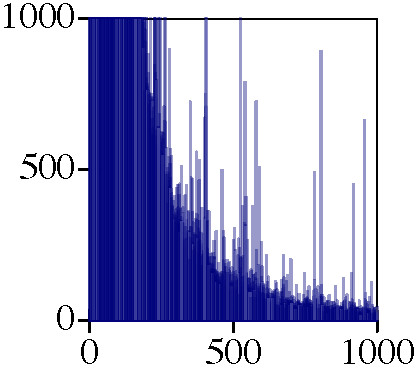
\includegraphics[width=0.4\columnwidth]{out/lines-distribution.pdf}
\end{minipage}\begin{minipage}{0.5\columnwidth}
  \textbf{Edit Range:}\\
  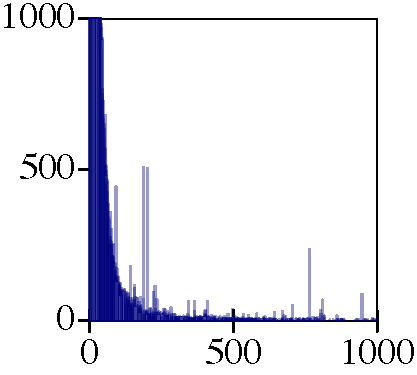
\includegraphics[width=0.4\columnwidth]{out/editrange-distribution.pdf}
\end{minipage}


%% ---
\subsection*{Table 3: Session Size}

See previous section for mean, stddev, median, and P99.

\begin{minipage}{0.5\columnwidth}
  \textbf{Timespan:}\\
  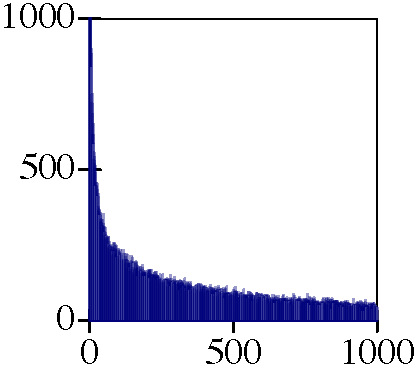
\includegraphics[width=0.4\columnwidth]{out/timespan-distribution.pdf}
\end{minipage}\begin{minipage}{0.5\columnwidth}
  \textbf{Event Count / Record Count:}\\
  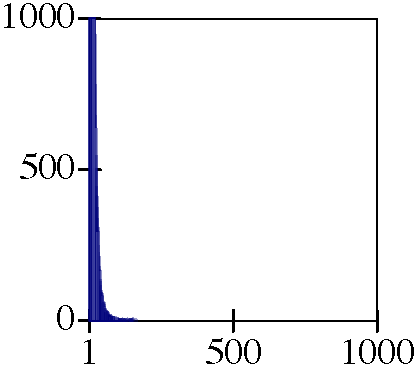
\includegraphics[width=0.4\columnwidth]{out/event-count-distribution.pdf}
\end{minipage}


%% ---
\subsection*{Table 4: Current Type Errors and Background Errors}

Lines 3-8 of \texttt{out/overview.txt}:

\begin{verbatim}
 72235735 total forced strict type errors, 37027281 in module,
 curr 1111178 in edit regions,
 olde 938500 in edit regions
 595137 total type errors, 289698 in module,
 curr 14917 non-stx + 16007 syntax in edit regions,
 olde 13836 non-stx + 28565 syntax in edit regions
\end{verbatim}

Current errors in edit range = (14917 + 16007) = 30924


%% ---
\subsection*{Figure 4: Overview of Type Analysis Modes}

Line 1 of \texttt{out/overview.txt} partitions logs by mode:

\begin{verbatim}
 1504736 total logs = 1341348 nocheck + 156883 nonstrict + 6505 strict
\end{verbatim}

Lines 9-13 of \texttt{out/overview.txt} partition sessions and report on upgrades and downgrades,
\emph{but} the final two numbers are incorrect (upgrade and downgrade) because they include
data from module switches:

\begin{verbatim}
 347598 sessions
  346956 single mode = 313509 nocheck + 32902 nonstrict + 545 strict
  512 multi mode projects
  341 mode upgrades
  320 mode downgrades
\end{verbatim}

There are 642 = (347598 - 346956) multi-mode sessions.

Correct up/down-grade numbers are in \texttt{out/downgrade-count.txt},
which is the output of \texttt{code/downgrade-count.rkt} after running
the following commands to generate data:

\begin{verbatim}
PLTSTDERR="error info@luau" racket prepare.rkt --mode divide-sessions
PLTSTDERR="error info@luau" racket prepare.rkt --mode session-query
PLTSTDERR="error info@luau" racket prepare.rkt --mode aggregate-te
\end{verbatim}

Output:

\verbatiminput{out/downgrade-count.txt}


%% ---
\subsection*{Figure 5: Type and Background Errors Grouped by Mode}

These plots come from \texttt{code/error-by-mode.rkt}, which uses
hard-coded data from \texttt{out/overview.txt}:

{ \newcommand{\labelbars}[1]{\begin{tabular}[t]{l@{}l} \raisebox{2ex}{\begin{tabular}[t]{r}\mnocheck{}\\\mnonstrict{}\\\mstrict{}\end{tabular}} & #1 \end{tabular}}
  \begin{tabular}[t]{cc}
    Type errors & Background errors \\
    \labelbars{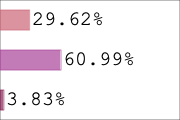
\includegraphics[width=0.20\columnwidth,valign=M]{out/error-by-mode-te.png}}
    & \labelbars{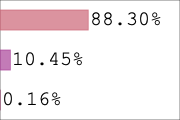
\includegraphics[width=0.20\columnwidth,valign=M]{out/error-by-mode-fs.png}}
  \end{tabular}
}


%% ---
\subsection*{Table 5: Specific Errors in Edit Range}

Output from \texttt{code/type-error-survival.rkt}
run on \texttt{code/type-error-survival-ss-*.rktd}
and then sorted alphabetically:

\begin{tabular}{lr@{~}r@{~}rr@{~}r@{~}rr@{~}r@{~}r}
  & \zerowidth{\mnocheck{}} & & & \zerowidth{\mnonstrict{}} & & & \zerowidth{\mstrict{}} & & \\
  & \rcell{Add} & \ycell{Keep} & \gcell{Drop} & \rcell{Add} & \ycell{Keep} & \gcell{Drop} & \rcell{Add} & \ycell{Keep} & \gcell{Drop} \\\hline
  CannotCallNonFunction & {0} & {0} & {0} & {12} & {2} & {13} & {1} & {0} & {1} \\
  CannotExtendTable & {0} & {0} & {0} & {6} & {8} & {1} & {0} & {0} & {1} \\
  CannotInferBinaryOperation & {0} & {0} & {0} & {0} & {1} & {0} & {5} & {6} & {6} \\
  CountMismatch & {0} & {0} & {0} & {184} & {42} & {157} & {9} & {2} & {9} \\
  DuplicateTypeDefinition & {0} & {0} & {0} & {1} & {0} & {0} & {0} & {0} & {0} \\
  ExtraInformation & {0} & {0} & {0} & {46} & {6} & {33} & {1} & {0} & {1} \\
  FunctionDoesNotTakeSelf & {0} & {0} & {0} & {3} & {4} & {1} & {0} & {0} & {0} \\
  FunctionExitsWithoutReturning & {0} & {0} & {0} & {6} & {1} & {5} & {7} & {3} & {5} \\
  GenericError & {0} & {0} & {0} & {177} & {47} & {149} & {5} & {0} & {8} \\
  IllegalRequire & {0} & {0} & {0} & {7} & {1} & {11} & {0} & {0} & {0} \\
  IncorrectGenericParameterCount & {0} & {0} & {0} & {0} & {0} & {0} & {1} & {0} & {1} \\
  MissingProperties & {0} & {0} & {0} & {8} & {3} & {6} & {5} & {3} & {3} \\
  ModuleHasCyclicDependency & {0} & {0} & {0} & {9} & {5} & {8} & {0} & {0} & {0} \\
  NotATable & {0} & {0} & {0} & {4} & {1} & {5} & {2} & {0} & {1} \\
  OccursCheckFailed & {0} & {0} & {0} & {0} & {0} & {0} & {0} & {0} & {1} \\
  OnlyTablesCanHaveMethods & {0} & {0} & {0} & {0} & {0} & {2} & {0} & {0} & {0} \\
  OptionalValueAccess & {0} & {0} & {0} & {21} & {45} & {15} & {4} & {2} & {4} \\
  SyntaxError & {0} & {0} & {8290} & {0} & {0} & {1149} & {0} & {0} & {29} \\
  TypeMismatch & {0} & {0} & {0} & {103} & {51} & {80} & {13} & {6} & {18} \\
  UnknownPropButFoundLikeProp & {0} & {0} & {0} & {20} & {17} & {13} & {0} & {0} & {0} \\
  UnknownProperty & {0} & {0} & {0} & {256} & {156} & {208} & {16} & {18} & {22} \\
  UnknownRequire & {0} & {0} & {0} & {43} & {30} & {37} & {5} & {3} & {3} \\
  UnknownSymbol & {0} & {0} & {0} & {1992} & {438} & {1797} & {38} & {18} & {35} \\
\end{tabular}


%% ---
\subsection*{Table 6: Type Error Popularity}

Output from \texttt{code/type-error-count.rkt}
run on \texttt{code/te-editrange-ss-*.rktd}.

This script produces output for all three modes: \mnocheck{}, \mnonstrict{}, and \mstrict{}.
The paper combines \mnonstrict{} and \mstrict{} into one table.

\subsubsection*{\mnocheck{}}

unused code IllegalRequire
unused code UnknownSymbol
unused code TypeMismatch
unused code NormalizationTooComplex
unused code DynamicPropertyLookupOnClassesUnsafe
unused code MissingUnionProperty
unused code UnknownProperty
unused code TypePackMismatch
unused code DuplicateTypeDefinition
unused code UnknownRequire
unused code TypesAreUnrelated
unused code MissingProperties
unused code FunctionExitsWithoutReturning
unused code CannotExtendTable
unused code FunctionDoesNotTakeSelf
unused code UnificationTooComplex
unused code GenericError
unused code NotATable
unused code OnlyTablesCanHaveMethods
unused code CodeTooComplex
unused code InternalError
unused code FunctionRequiresSelf
unused code UnknownPropButFoundLikeProp
unused code CannotInferBinaryOperation
unused code IncorrectGenericParameterCount
unused code OptionalValueAccess
unused code DuplicateGenericParameter
unused code CountMismatch
unused code OccursCheckFailed
unused code DeprecatedApiUsed
unused code CannotCallNonFunction
unused code ModuleHasCyclicDependency
unused code SwappedGenericTypeParameter
unused code ExtraInformation
NEVER APPEAR: (IllegalRequire UnknownSymbol TypeMismatch NormalizationTooComplex DynamicPropertyLookupOnClassesUnsafe MissingUnionProperty UnknownProperty TypePackMismatch DuplicateTypeDefinition UnknownRequire TypesAreUnrelated MissingProperties FunctionExitsWithoutReturning CannotExtendTable FunctionDoesNotTakeSelf UnificationTooComplex GenericError NotATable OnlyTablesCanHaveMethods CodeTooComplex InternalError FunctionRequiresSelf UnknownPropButFoundLikeProp CannotInferBinaryOperation IncorrectGenericParameterCount OptionalValueAccess DuplicateGenericParameter CountMismatch OccursCheckFailed DeprecatedApiUsed CannotCallNonFunction ModuleHasCyclicDependency SwappedGenericTypeParameter ExtraInformation)

\begin{tabular}{lr}
  \code{SyntaxError} & \pct{100.00} \\
\end{tabular}

\subsubsection*{\mnonstrict{}}

unused code NormalizationTooComplex
unused code DynamicPropertyLookupOnClassesUnsafe
unused code TypePackMismatch
unused code UnificationTooComplex
unused code CodeTooComplex
unused code InternalError
unused code FunctionRequiresSelf
unused code IncorrectGenericParameterCount
unused code DuplicateGenericParameter
unused code OccursCheckFailed
unused code DeprecatedApiUsed
unused code SwappedGenericTypeParameter
NEVER APPEAR: (NormalizationTooComplex DynamicPropertyLookupOnClassesUnsafe TypePackMismatch UnificationTooComplex CodeTooComplex InternalError FunctionRequiresSelf IncorrectGenericParameterCount DuplicateGenericParameter OccursCheckFailed DeprecatedApiUsed SwappedGenericTypeParameter)

\begin{tabular}{lr}
  \code{UnknownSymbol} & \pct{62.13} \\
  \code{SyntaxError} & \pct{15.42} \\
  \code{UnknownProperty} & \pct{8.28} \\
  \code{UnknownRequire} & \pct{3.13} \\
  \code{TypeMismatch} & \pct{2.44} \\
  \code{CountMismatch} & \pct{2.26} \\
  \code{OptionalValueAccess} & \pct{2.07} \\
  \code{GenericError} & \pct{2.06} \\
  \code{UnknownPropButFoundLikeProp} & \pct{0.44} \\
  \code{CannotExtendTable} & \pct{0.42} \\
  \code{ExtraInformation} & \pct{0.32} \\
  \code{ModuleHasCyclicDependency} & \pct{0.23} \\
  \code{IllegalRequire} & \pct{0.20} \\
  \code{NotATable} & \pct{0.15} \\
  \code{CannotCallNonFunction} & \pct{0.15} \\
  \code{MissingProperties} & \pct{0.09} \\
  \code{FunctionExitsWithoutReturning} & \pct{0.07} \\
  \code{FunctionDoesNotTakeSelf} & \pct{0.07} \\
  \code{MissingUnionProperty} & \pct{0.02} \\
  \code{CannotInferBinaryOperation} & \pct{0.02} \\
  \code{OnlyTablesCanHaveMethods} & \pct{0.01} \\
  \code{DuplicateTypeDefinition} & \pct{0.00} \\
  \code{TypesAreUnrelated} & \pct{0.00} \\
\end{tabular}

\subsubsection*{\mstrict{}}

unused code NormalizationTooComplex
unused code DynamicPropertyLookupOnClassesUnsafe
unused code MissingUnionProperty
unused code TypePackMismatch
unused code DuplicateTypeDefinition
unused code FunctionDoesNotTakeSelf
unused code UnificationTooComplex
unused code OnlyTablesCanHaveMethods
unused code CodeTooComplex
unused code InternalError
unused code FunctionRequiresSelf
unused code DuplicateGenericParameter
unused code DeprecatedApiUsed
unused code SwappedGenericTypeParameter
NEVER APPEAR: (NormalizationTooComplex DynamicPropertyLookupOnClassesUnsafe MissingUnionProperty TypePackMismatch DuplicateTypeDefinition FunctionDoesNotTakeSelf UnificationTooComplex OnlyTablesCanHaveMethods CodeTooComplex InternalError FunctionRequiresSelf DuplicateGenericParameter DeprecatedApiUsed SwappedGenericTypeParameter)

\begin{tabular}{lr}
  \code{UnknownSymbol} & \pct{23.97} \\
  \code{TypeMismatch} & \pct{20.46} \\
  \code{UnknownProperty} & \pct{18.88} \\
  \code{SyntaxError} & \pct{9.31} \\
  \code{CannotInferBinaryOperation} & \pct{6.94} \\
  \code{MissingProperties} & \pct{4.04} \\
  \code{FunctionExitsWithoutReturning} & \pct{2.99} \\
  \code{OptionalValueAccess} & \pct{2.99} \\
  \code{CountMismatch} & \pct{2.99} \\
  \code{UnknownRequire} & \pct{2.37} \\
  \code{GenericError} & \pct{2.28} \\
  \code{NotATable} & \pct{1.32} \\
  \code{ExtraInformation} & \pct{0.35} \\
  \code{UnknownPropButFoundLikeProp} & \pct{0.26} \\
  \code{IllegalRequire} & \pct{0.18} \\
  \code{IncorrectGenericParameterCount} & \pct{0.18} \\
  \code{CannotCallNonFunction} & \pct{0.18} \\
  \code{TypesAreUnrelated} & \pct{0.09} \\
  \code{CannotExtendTable} & \pct{0.09} \\
  \code{OccursCheckFailed} & \pct{0.09} \\
  \code{ModuleHasCyclicDependency} & \pct{0.09} \\
\end{tabular}


\subsubsection*{Internal Limits, Code Too Complex}

Data from \texttt{out/ctc-info.txt}, which comes from
\texttt{prepare.rkt --mode main}:

{\footnotesize
\verbatiminput{out/ctc-info.txt}
}


%% ---
\subsection*{Figure 6: Type Error Density}

Plot output from \texttt{code/error-count.rkt}
on \texttt{out/error-density-ss-*.rktd}.
(It also prints text output.):

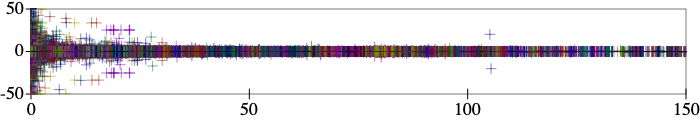
\includegraphics[width=0.8\columnwidth]{out/error-count-nocheck-row--te-density-diff.png}

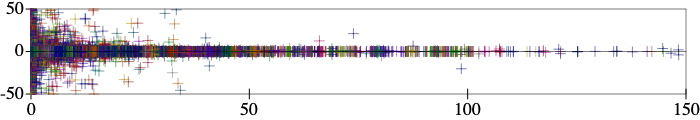
\includegraphics[width=0.8\columnwidth]{out/error-count-nonstrict-row--te-density-diff.png}

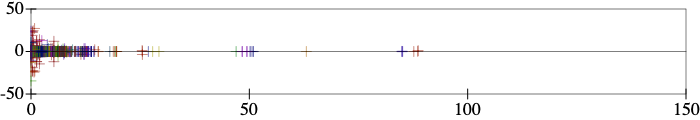
\includegraphics[width=0.8\columnwidth]{out/error-count-strict-row--te-density-diff.png}


\subsection*{Figure 7: Edits and Number of Errors}

From reordered text output from \texttt{code/error-count.rkt}
on \texttt{out/error-density-ss-*.rktd}.
Here is the raw, unsorted output:

\begin{verbatim}
TE
  nocheck & 48378 & (\pct{46.83}) & 9440 & [\pct{9.14}] & 45479 & [\pct{44.03}] \\
FS
  nocheck & 270763 & (\pct{36.99}) & 238696 & [\pct{32.61}] & 222588 & [\pct{30.41}] \\
TE mod
  nocheck & 20085 & (\pct{49.83}) & 906 & [\pct{2.25}] & 19317 & [\pct{47.92}] \\
FS mod
  nocheck & 259865 & (\pct{39.09}) & 175643 & [\pct{26.42}] & 229271 & [\pct{34.49}] \\
TE
  nonstrict & 19491 & (\pct{39.63}) & 9567 & [\pct{19.45}] & 20121 & [\pct{40.91}] \\
FS
  nonstrict & 35330 & (\pct{37.28}) & 29483 & [\pct{31.11}] & 29955 & [\pct{31.61}] \\
TE mod
  nonstrict & 13030 & (\pct{40.22}) & 5513 & [\pct{17.02}] & 13852 & [\pct{42.76}] \\
FS mod
  nonstrict & 33988 & (\pct{39.74}) & 20738 & [\pct{24.25}] & 30798 & [\pct{36.01}] \\
TE
  strict & 733 & (\pct{39.18}) & 368 & [\pct{19.67}] & 770 & [\pct{41.15}] \\
FS
  strict & 574 & (\pct{33.71}) & 561 & [\pct{32.94}] & 568 & [\pct{33.35}] \\
TE mod
  strict & 419 & (\pct{39.31}) & 230 & [\pct{21.58}] & 417 & [\pct{39.12}] \\
FS mod
  strict & 488 & (\pct{36.53}) & 344 & [\pct{25.75}] & 504 & [\pct{37.72}] \\
\end{verbatim}



\end{document}
